\documentclass{beamer}

\mode<presentation>
{\usetheme{boxes}}

\usepackage{array}
\usepackage{times}
\usepackage{graphicx}
\usepackage{hyperref}
\usepackage{listings}
\usepackage{relsize}
\usepackage{ragged2e}
\usepackage[T1]{fontenc}

\lstdefinestyle{customc}{
  belowcaptionskip=1\baselineskip,
  breaklines=true,
  frame=L,
  xleftmargin=\parindent,
  language=C,
  showstringspaces=false,
  basicstyle=\footnotesize\ttfamily,
  keywordstyle=\bfseries\color{green!40!black},
  commentstyle=\itshape\color{purple!40!black},
  identifierstyle=\color{blue},
  stringstyle=\color{red},
}
\lstdefinestyle{custombash}{
  belowcaptionskip=1\baselineskip,
  breaklines=true,
  frame=L,
  xleftmargin=\parindent,
  language=bash,
  basicstyle=\footnotesize\ttfamily,
  showstringspaces=false,
  commentstyle=\itshape\color{purple!40!black},
  keywordstyle=\itshape\color{green!40!black},
  identifierstyle=\color{blue},
  stringstyle=\color{orange},
}

\usebackgroundtemplate
{
  \hbox to \paperwidth{\hfil
\includegraphics[width=4in,
      height=\paperheight]{wildcat_transparent.jpg}\hfil}
}

\title{PHYS 105 Lecture 10: Gaussians, Dynamic Displays}
\author{Tom McClintock \\
	Dept. of Physics\\
	University of Arizona
}
\date{\today}

\begin{document}

\begin{frame}
  \titlepage
\end{frame}

\begin{frame}
  \frametitle{Last time}
  \begin{itemize}
    \item File I/O
    \item Histograms
  \end{itemize}
\end{frame}

\begin{frame}
  \frametitle{This time}
  \begin{itemize}
    \item Drawing a Gaussian
    \item Dynamic displays
  \end{itemize}
\end{frame}

\begin{frame}
  \frametitle{Gaussian}
  A Guassian (aka normal) distribution is a special one for physicists.
  This is because it is the most common distribution for measurements.\\
  \centering
  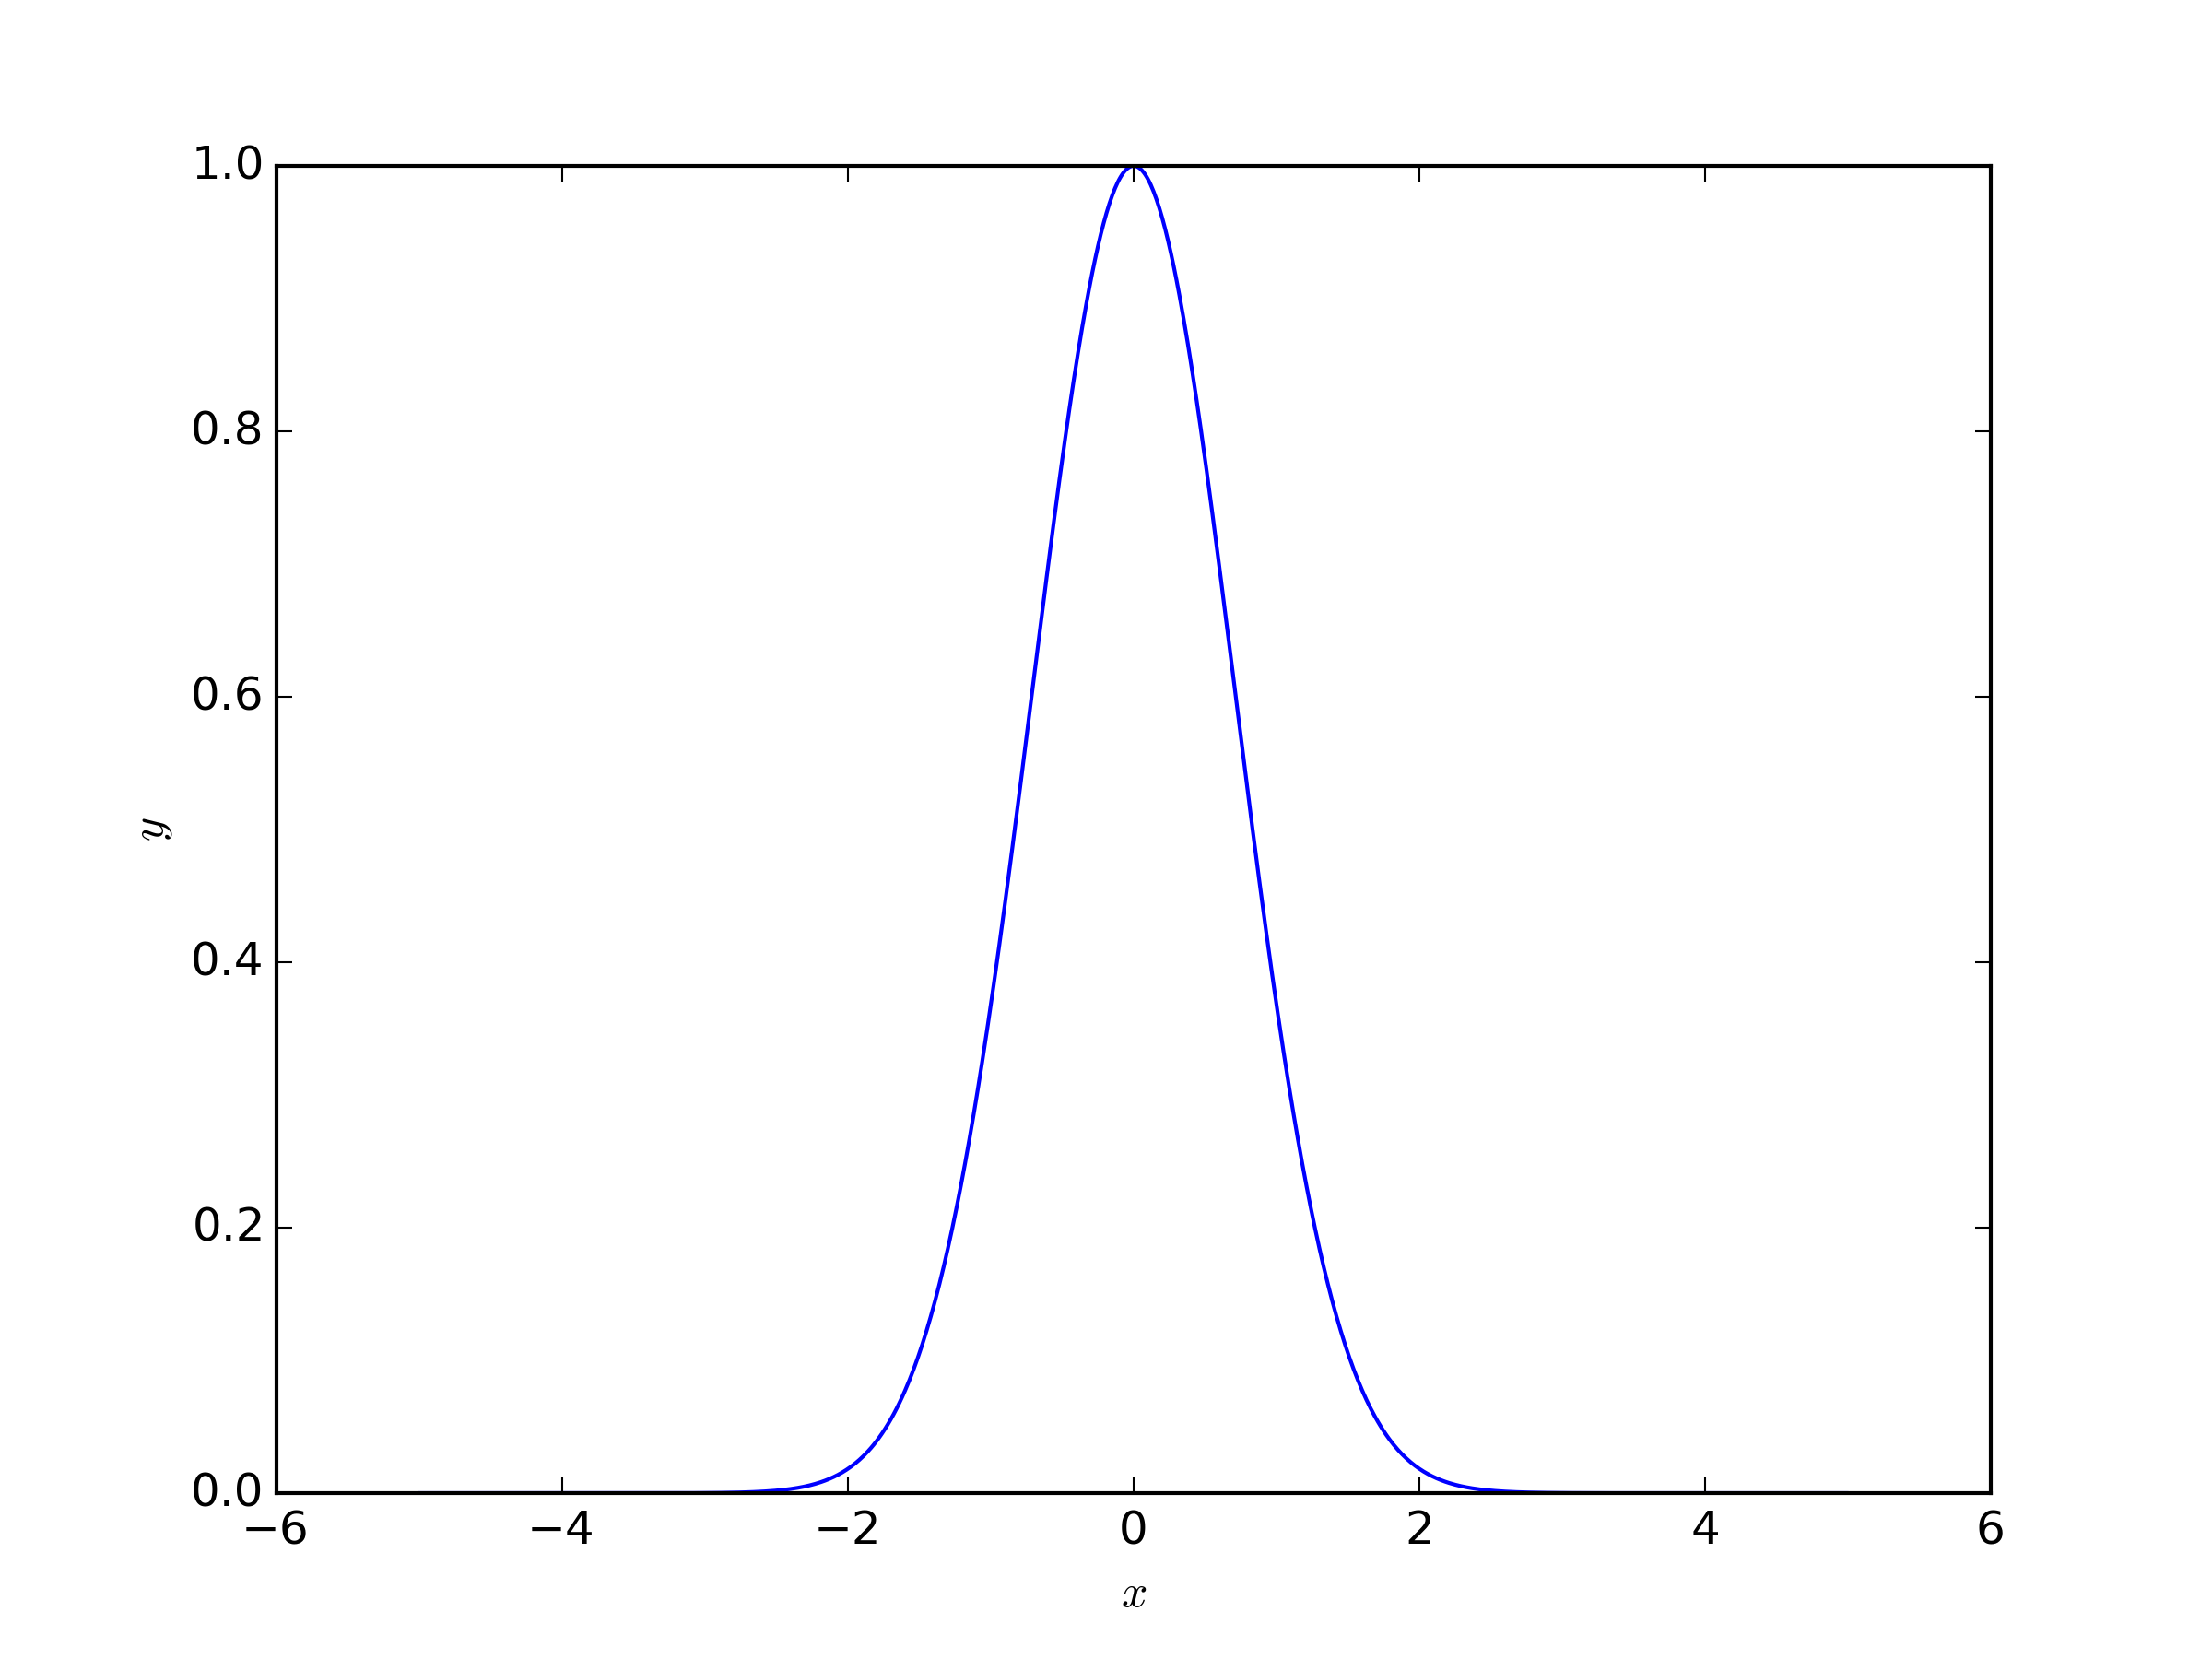
\includegraphics[width=0.7\textwidth]{gaussian.png}
\end{frame}

\begin{frame}[fragile,allowframebreaks]
  \frametitle{draw\_gaussian.c}
  This is a graphical version of the program we did two weeks ago.
  \lstinputlisting[style=customc]{draw_gaussian.c}
\end{frame}

\begin{frame}[fragile]
  \frametitle{Dynamic displays}
  A key part of a simulation is being able to visualize data in real time, but
  in order to do this we need to be able to draw in real time.\\
  Add the following lines inside the \textbf{for} loop of the previous program:
  \begin{lstlisting}[style=customc]
    delay_plot(20);
    flush_plot();
  \end{lstlisting}
\end{frame}

\begin{frame}[fragile]
  \frametitle{delay\_plot()}
  What is the purpose of these two lines?
  \begin{lstlisting}[style=customc]
    delay_plot(20);
    flush_plot();
  \end{lstlisting}
  First, the \textbf{delay\_plot()} call adds a delay in milliseconds
  when that function is called. So \textbf{delay\_plot(20)} will cause a 
  20 millisecond delay.\\
  Second, by adding the \textbf{flush\_plot()} inside the loop, an updated
  display is drawn each time through. So the program draws a tiny part of the
  line, and draws to screen.\\
  This has the effect of animating the drawing process!
\end{frame}

\begin{frame}
  \frametitle{Drawing a dot}
  Many of the simulations we will do in this class will involve moving
  a dot along a screen. The next program shows how you can draw a
  point of any number of vertices on the screen.
\end{frame}

\begin{frame}[fragile,allowframebreaks]
  \frametitle{draw\_dot.c}
  \lstinputlisting[style=customc]{draw_dot.c}
\end{frame}

\begin{frame}
  \frametitle{In class assignment}
  \begin{enumerate}
    \item Try chaning \textbf{pVertex}, \textbf{pColor}, and
      \textbf{pStyle} in the draw\_dot.c program.
    \item Make the dot move from the left side of the screen
      to the right side of the screen smoothly. Hint: you need
      a loop.
    \item (If you have time) Have the dot follow the path of the Gaussian!
  \end{enumerate}
\end{frame}

\begin{frame}
  \frametitle{Next time}
  \begin{itemize}
  \item Simulating a bouncing ball
  \end{itemize}

\end{frame}

\begin{frame}
  \frametitle{HW 6 - photon off of a mirror due in two weeks}
  Create a program that bounces a photon (dot) off of a mirror. Have
  the photon come in from the top left corner, hit the mirror in the center,
  and leave through the top right corner.
\end{frame}

\end{document}